\documentclass{article}

% NeurIPS 2024 style — download neurips_2024.sty from:
% https://neurips.cc/Conferences/2024/PaperInformation/StyleFiles
\usepackage[final]{neurips_2024}

\usepackage[utf8]{inputenc}
\usepackage[T1]{fontenc}
\usepackage{hyperref}
\usepackage{url}
\usepackage{booktabs}
\usepackage{amsfonts}
\usepackage{amsmath}
\usepackage{amssymb}
\usepackage{nicefrac}
\usepackage{microtype}
\usepackage{xcolor}
\usepackage{graphicx}
\usepackage{subcaption}
\usepackage{multirow}
\usepackage{makecell}
\usepackage{array}
\usepackage{colortbl}
\usepackage{wrapfig}
\usepackage{natbib}
\usepackage{cleveref}

% ── Colour helpers ─────────────────────────────────────────────────────────────
\definecolor{bestcol}{RGB}{198,239,206}
\definecolor{warncolor}{RGB}{255,235,156}
\newcommand{\best}[1]{\cellcolor{bestcol}\textbf{#1}}
\newcommand{\second}[1]{\cellcolor{warncolor}{#1}}

% ── Title & authors ────────────────────────────────────────────────────────────
\title{MemeSonic: Unified Affective Meme Audio Generation\\and Tri-Modal Alignment}

\author{%
  Yiqiao Huang \And Hongbee Park \And Ruyi Yang \\[2pt]
  MIT MAS.S60 / 6.S985 — Multimodal AI, Spring 2026
}

\begin{document}
\maketitle

% ── Pipeline overview figure ───────────────────────────────────────────────────
% Place the pipeline diagram (from slide p.9) as figures/pipeline.png
\begin{figure}[t]
  \centering
  % Uncomment once figures/pipeline.png is added:
  % 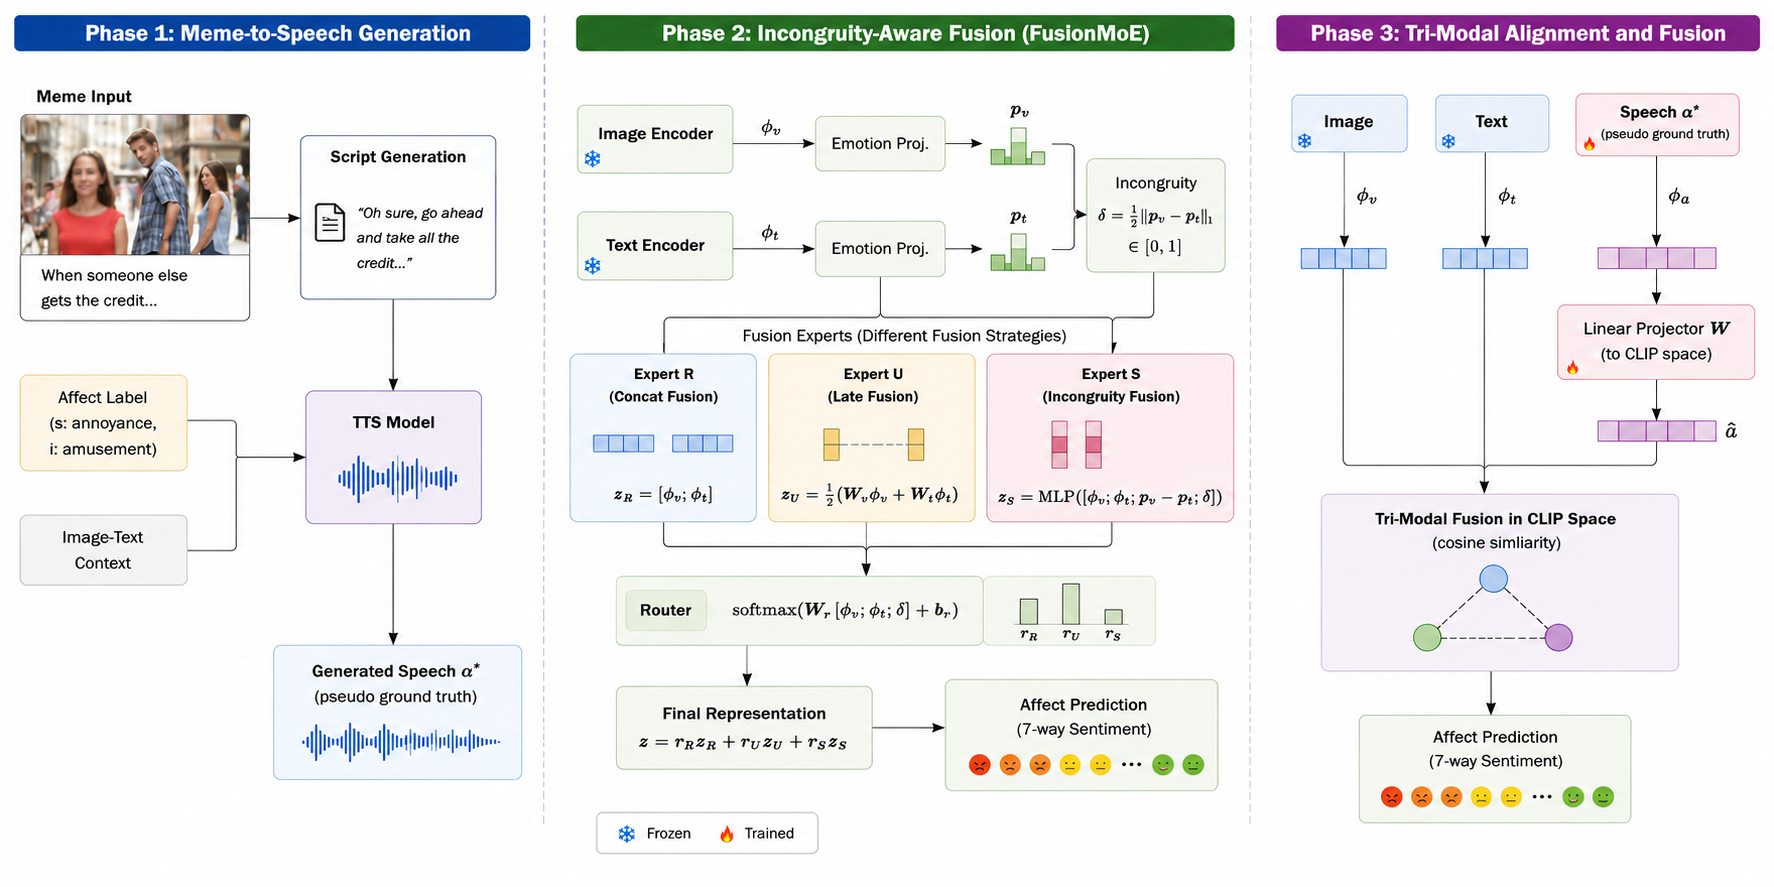
\includegraphics[width=\linewidth]{figures/pipeline.png}
  \fbox{\parbox{0.95\linewidth}{\centering\vspace{2em}
    \textit{[Figure: MemeSonic system overview — Meme Input $\to$ CLIP Encoders $\to$
    Incongruity Score $\to$ MMOE Routing $\to$ Labels \& Fused Embedding $\to$
    LLM Adapter / Open-source Adapter $\to$ Synthesized Audio]}
  \vspace{2em}}}
  \caption{MemeSonic system overview. The framework decomposes image and text into independent
  emotion distributions, computes a cross-modal incongruity score, routes each sample to the
  appropriate fusion expert, and translates the fused representation into prosodically expressive
  audio via two generation paths.}
  \label{fig:pipeline}
\end{figure}

% ── Sections ───────────────────────────────────────────────────────────────────
\begin{abstract}
Memes derive their communicative power not from semantic alignment between image and text, but from
\emph{intentional incongruity}—a smiling dog in a burning room, a deadpan face paired with absurdist
caption. Yet existing multimodal systems assume modalities agree and consequently collapse on the
conflict-dominant, non-literal language that defines meme affect.
We present \textbf{MemeSonic}, a unified framework for meme affective understanding and expressive
audio generation, built on a central premise: the \emph{incongruity} between image and text is not
noise to suppress but a differentiable signal to model.
To capture this signal, our framework first introduces independent multimodal encoding: image and text
are each mapped to their own emotion distributions, and a continuous cross-modal incongruity score is
derived from their divergence—making the tension between modalities an explicit, learnable feature
rather than an artifact to discard.
This incongruity score then drives \emph{Incongruity-Aware Mixture-of-Experts (MMOE) Fusion} for
affective classification. Across ten tasks on three meme benchmarks (MET-Meme, Memotion~7k,
MMSD~2.0), Incongruity Fusion achieves the best Macro-F1 on five tasks and MMOE achieves best on
four, outperforming standard fusion baselines by up to \textbf{+12.1\%} accuracy.
Beyond classification, we propagate the same incongruity signal into audio generation via an
\emph{Incongruity-to-Prosody Adapter}, enabling expressive speech synthesis that mirrors the
affective tension of the source meme. Human evaluation (n=84) shows MemeSonic achieves AMOS~3.95
vs.\ 1.68 for Vanilla TTS, with 84.5\% preference in A/B tests.
Finally, to assess whether audio carries affective signal beyond image and text, we conduct a
controlled tri-modal alignment experiment using Emotion2Vec embeddings, finding that naive
heterogeneous fusion yields zero modal contribution, while a learned linear projector bridges the
modality gap and raises sentiment accuracy from 27\% to 82\%—confirming that audio is a
non-redundant affective modality once properly aligned.
\end{abstract}

\section{Introduction}

Memes are among the most prolific forms of digital communication, yet they remain deeply challenging
for multimodal AI. Unlike image-caption pairs where visual and textual content reinforce each other,
memes deliberately exploit \emph{incongruity}—a serene image paired with a desperate caption, a
cheerful face accompanying nihilistic text. This cross-modal conflict is not noise to be filtered; it is
the semantic mechanism through which humor, sarcasm, and irony are constructed. As a result, standard
multimodal models that assume or enforce cross-modal agreement systematically fail on meme affect.

The challenge compounds when we ask: \emph{how should a meme sound?} Human narrators instinctively
adjust pitch, pace, and emotional coloring when reading meme text aloud—leaning into irony,
exaggerating deadpan delivery, or escalating expressive intensity to match the visual absurdity. Current
text-to-speech (TTS) systems have no access to this pragmatic context; they generate audio from text
semantics alone, missing the affective layer encoded in the image-text relationship. This produces audio
that is semantically correct but expressively hollow—natural in isolation, inappropriate for the meme.

A third, underexplored dimension is the audio modality itself: once a voiced meme exists, does the
prosodic rendering add information beyond what image and text already communicate? Do different
emotional renderings of the same script change how viewers perceive sentiment and intention? These
questions have practical implications for accessible content, meme retrieval, and affective computing,
yet no prior work has systematically studied tri-modal (image, text, audio) interaction in the meme domain.

\textbf{In this paper}, we introduce \textbf{MemeSonic}, a unified framework that addresses meme
understanding and expressive audio generation jointly. Our contributions are:

\begin{enumerate}
  \item \textbf{Explicit Affect Decomposition.} We decompose meme understanding into independent
    per-modality emotion distributions and compute a continuous \emph{incongruity score} that
    quantifies cross-modal conflict. This turns the incongruity—previously treated as noise—into an
    explicit, differentiable signal available throughout the pipeline.

  \item \textbf{Incongruity-Aware MMOE Fusion.} We propose a Mixture-of-Experts fusion mechanism
    whose router is conditioned on the incongruity signal. Three expert strategies handle distinct
    interaction types: Redundancy (Concat), Uniqueness (Late Fusion), and Synergy (Incongruity
    Fusion). This is fundamentally different from standard MoE systems that route on task difficulty
    or data statistics; our router encodes the \emph{semantic relationship} between modalities.

  \item \textbf{Meme-to-Speech Pipeline.} We translate the
    fused affective representation into expressive audio via an adapter that conditions TTS synthesis
    on the incongruity score, enabling prosodic variance to reflect not just the text sentiment but
    the cross-modal pragmatic intent of the meme.

  \item \textbf{Tri-Modal Alignment Study.} We conduct a controlled experiment across a 3$\times$3
    prosody grid (stability $\times$ style) to quantify whether audio modality contributes independent
    affective information beyond image-text fusion. Using Emotion2Vec embeddings and a learned linear
    projector to bridge modality spaces, we provide the first systematic evidence that (a) audio
    carries non-redundant emotional signal (KL divergence: $V$\,$\leftrightarrow$\,$A$ = 1.14 vs.\
    $V$\,$\leftrightarrow$\,$T$ = 0.69), and (b) the failure of naive fusion is a \emph{modality gap
    problem}, not an absence of information.
\end{enumerate}

Across 10 classification tasks on three benchmarks (MET-Meme, Memotion 7k, MMSD 2.0), our
Incongruity-Aware Fusion achieves the best Macro-F1 on tasks dominated by non-literal language
(metaphor +87.6\%, humour +12.1\% over Late Fusion). Human evaluation of generated audio
(n=84 ratings) shows MemeSonic achieves AMOS 3.95 vs.\ 1.68 for Vanilla TTS, with 84.5\%
preference over the vanilla baseline—demonstrating that incongruity-aware conditioning substantially
improves pragmatic appropriateness without sacrificing naturalness.

% \section{Related Work}

% \subsection{Meme Understanding and Affect Analysis}
% Early meme analysis focused on hateful content detection~\citep{kiela2020hateful}, framing the problem
% as binary classification over image-text pairs with concatenated unimodal representations. MemeCLIP~\citep{shi2024memeclip} extended this to contrastive pre-training with meme-specific augmentations.
% MER-Bench and related surveys~\citep{sharma2020semeval,caton2023memotion} introduced multi-task sentiment, humor, and offensiveness labels for Memotion 7k and MMSD 2.0~\citep{mmsd2}, providing standardized benchmarks we adopt. A critical limitation shared by all these works is that they treat image and text as semantically synergistic—averaging or concatenating representations—and do not model the \emph{intentional conflict} that gives memes their expressive character.

% \subsection{Multimodal Fusion with Conflict Modeling}
% CLIP~\citep{radford2021clip} and BLIP~\citep{li2022blip} achieve strong image-text alignment by
% assuming cross-modal agreement; ALIGN~\citep{jia2021align} scales this with noisy web data. ImageBind~\citep{girdhar2023imagebind} extends alignment to six modalities via shared embedding spaces. These
% models excel on literal, descriptive content but struggle on memes where visual and textual affect
% diverge. MULT~\citep{tsai2019mult} introduces cross-modal attention for sentiment analysis in video
% but operates on synchronized temporal streams rather than static image-text pairs. MMOE~\citep{yu2024mmoe} proposes interaction-type-aware expert routing for multimodal fusion, which we adapt and
% extend with explicit incongruity conditioning. Unlike MMOE's learned router, our router is directly
% conditioned on a computed incongruity score, giving it an inductive bias toward cross-modal conflict.

% \subsection{Humor and Incongruity in Computational Humor}
% The incongruity-resolution theory of humor~\citep{suls1972two} posits that humor arises from the
% detection and resolution of a perceived incongruity. Computational work has operationalized this in
% text~\citep{yang2015humor} and image-text pairs~\citep{hessel2022meme}, but has rarely embedded
% it as an architectural component in fusion models. \citet{cai2019multi} use a hierarchical model for
% meme sentiment but do not explicitly score or route on incongruity. Our work is the first to use a
% differentiable incongruity score as a routing signal in a multi-expert fusion framework.

% \subsection{Expressive and Controllable Text-to-Speech}
% Neural TTS has advanced rapidly from Tacotron~\citep{wang2017tacotron} and FastSpeech~\citep{ren2021fastspeech} to StyleTTS2~\citep{li2024styletts2}, which models style as a latent variable
% enabling fine-grained prosody control. Emotion-conditioned TTS systems~\citep{lei2022emotion} transfer
% emotional styles from reference audio. ElevenLabs provides commercial TTS with \texttt{voice\_settings}
% parameters (stability, style) that offer limited but usable prosody control. Emotion2Vec~\citep{ma2023emotion2vec} extracts speech emotion embeddings trained on emotional speech corpora. None of these
% systems have been adapted to meme-specific pragmatic control, where the input is not a desired emotion
% label but a cross-modal incongruity signal derived from image-text analysis.

% \subsection{Audio in Multimodal Understanding}
% ImageBind~\citep{girdhar2023imagebind} aligns audio with other modalities via contrastive training on
% environmental sounds (AudioSet), achieving near-perfect text-audio retrieval on natural sounds but
% essentially zero performance on TTS-generated emotional speech (Top-1 $\approx$ 0.00 in our probing
% experiments). This \emph{modality gap}—the incompatibility between pretrained embedding spaces from
% different training regimes—is a known challenge in multimodal learning~\citep{liang2022mind}. We study
% this gap empirically in the meme audio domain and propose a linear projector bridge as a diagnostic
% tool, contributing to the understanding of when and why late fusion fails.

% \paragraph{How our work differs.}
% To our knowledge, MemeSonic is the first system to (1) model cross-modal incongruity as an explicit
% differentiable signal for both understanding and generation; (2) condition TTS prosody on this
% incongruity score rather than discrete emotion labels; and (3) conduct a controlled tri-modal alignment
% study in the meme domain, separating the contribution of audio modality from the modality gap problem.

\section{Problem Statement}

\paragraph{Notation.}
Let a meme be a triplet $\mathcal{M} = (v, t, a)$ where $v \in \mathcal{V}$ is the image,
$t \in \mathcal{T}$ is the overlaid text or caption, and $a \in \mathcal{A}$ is the synthesized
voiceover audio. In the understanding phase (Phase 1), $a$ is absent; in the generation phase (Phase 2),
$a$ is the output. Let $y^{(s)} \in \mathcal{Y}_s$ and $y^{(i)} \in \mathcal{Y}_i$ denote the ground-truth sentiment and intention labels respectively.

\paragraph{Phase 1 — Affective Understanding.}
Given $(v, t)$, we seek a function
$f: \mathcal{V} \times \mathcal{T} \rightarrow \mathcal{Y}_s \times \mathcal{Y}_i$
that correctly predicts sentiment and intention. Standard multimodal fusion defines:
\begin{equation}
  \hat{y} = \arg\max_y\; g\bigl(\phi_v(v),\, \phi_t(t)\bigr)
\end{equation}
where $\phi_v, \phi_t$ are frozen image and text encoders and $g$ is a fusion function. The key
challenge is that for memes, $\phi_v(v)$ and $\phi_t(t)$ may point to \emph{opposite} regions of
the emotion space, so naïve averaging suppresses rather than captures the affective content.

We formalize the incongruity signal as:
\begin{equation}
  \delta(v,t) = \bigl\|\, p_v - p_t \,\bigr\|_1
  \quad \in [0, 2]
\end{equation}
where $p_v, p_t \in \Delta^C$ are the per-modality emotion probability distributions over $C$
sentiment classes, obtained by projecting each encoder output onto a set of emotion prototype vectors.
A high $\delta$ indicates that image and text encode conflicting emotional content.

\paragraph{Phase 2 — Expressive Audio Generation.}
Given the fused affective representation $z = h(v, t, \delta) \in \mathbb{R}^d$ and a script
$s$ derived from the meme text, we seek a TTS function
$\Psi: \mathcal{T} \times \mathbb{R}^d \rightarrow \mathcal{A}$
that synthesizes audio whose prosodic profile matches the meme's pragmatic intent—not just its text
sentiment. The objective is:
\begin{equation}
  \Psi^* = \arg\max_\Psi\; \mathbb{E}_{(v,t,a^*)\sim\mathcal{D}}\bigl[\,
    \text{sim}\bigl(\Psi(s,z),\; a^*\bigr) +
    \lambda\cdot\text{AMOS}\bigl(\Psi(s,z)\bigr)
  \bigr]
\end{equation}
where $a^*$ is a pseudo ground-truth audio (closed-source TTS output), $\text{sim}(\cdot,\cdot)$ is
embedding cosine similarity, and AMOS is the human appropriateness rating.

\paragraph{Tri-Modal Alignment Study (RQ).}
For the diagnostic study, we additionally ask: given $a$, does audio contribute non-redundant
affective information to the prediction of $y^{(s)}$?
\begin{equation}
  \text{RQ:}\quad \text{Acc}\bigl(f(v,t,a)\bigr) \overset{?}{>} \text{Acc}\bigl(f(v,t)\bigr)
\end{equation}
and whether the failure of naive tri-modal fusion is attributable to a modality-space mismatch rather
than an absence of signal in $a$.

\section{Proposed Method}

MemeSonic is organized into two phases (Figure~\ref{fig:pipeline}): (1) Incongruity-Aware
Multimodal Understanding, which produces a structured affective representation of the meme;
and (2) Meme-to-Speech Generation, which translates this representation into expressively appropriate audio.

\subsection{Phase 1: Incongruity-Aware Multimodal Understanding}

\subsubsection{Explicit Affect Decomposition}
We encode the meme image $v$ with the CLIP image encoder $\phi_v$ and text $t$ with the CLIP text
encoder $\phi_t$, both frozen. Each encoder output is projected onto a set of $C$ emotion prototype
vectors $\{\mathbf{e}_c\}_{c=1}^C$ derived from CLIP text encodings of emotion label descriptions
(e.g., ``a happy and joyful image''):
\begin{equation}
  p^{(\cdot)}_c = \frac{\exp\!\bigl(\phi_{(\cdot)}(\cdot)^\top \mathbf{e}_c / \tau\bigr)}
                       {\sum_{j=1}^C \exp\!\bigl(\phi_{(\cdot)}(\cdot)^\top \mathbf{e}_j / \tau\bigr)}
\end{equation}
yielding emotion distributions $p_v, p_t \in \Delta^C$ for image and text respectively, where
$\tau$ is a temperature parameter. The incongruity score is:
\begin{equation}
  \delta(v,t) = \tfrac{1}{2}\,\|p_v - p_t\|_1 \;\in [0,1]
  \label{eq:incong}
\end{equation}
A value near 0 indicates emotional alignment (redundancy); a value near 1 indicates strong conflict
(synergy/incongruity). This scalar is differentiable with respect to the projection parameters and
is used throughout both phases.

\subsubsection{MMOE Fusion with Incongruity Routing}
\label{sec:mmoe}
Rather than applying a fixed fusion strategy, we route each sample to one of three expert fusion
modules based on its incongruity score $\delta$:

\textbf{Expert R (Redundancy)} handles samples where image and text are emotionally aligned
($\delta$ low). It concatenates the projected image and text embeddings:
$z_R = [\phi_v(v);\, \phi_t(t)]$, leveraging shared information.

\textbf{Expert U (Uniqueness)} handles samples where one modality dominates. It applies late fusion
via a learned weighted combination:
$z_U = \alpha \phi_v(v) + (1-\alpha) \phi_t(t)$, preserving modality-specific contributions.

\textbf{Expert S (Synergy)} handles high-incongruity samples. It applies Incongruity Fusion:
\begin{equation}
  z_S = \text{MLP}\bigl([\phi_v(v);\, \phi_t(t);\, p_v - p_t;\, \delta]\bigr)
\end{equation}
directly encoding the conflict vector $p_v - p_t$ and scalar $\delta$ into the representation.

The router is a single linear layer conditioned on $[\phi_v(v);\, \phi_t(t);\, \delta]$:
\begin{equation}
  \mathbf{r} = \text{softmax}\bigl(W_r [\phi_v(v);\, \phi_t(t);\, \delta] + b_r\bigr)
\end{equation}
The final fused representation is a soft mixture:
\begin{equation}
  z = r_R \cdot z_R + r_U \cdot z_U + r_S \cdot z_S
\end{equation}
followed by a task-specific linear classifier. During training, we use a two-objective loss:
$\mathcal{L} = \mathcal{L}_\text{cls}(z, y) + \lambda \mathcal{L}_\text{gate}(\mathbf{r}, \mathbf{r}^*)$,
where $\mathbf{r}^*$ are soft gate labels derived from the per-sample performance of the trained Concat
and Late Fusion experts.

\subsection{Phase 2: Meme-to-Speech Generation}

\subsubsection{Script Generation}
Given the meme image and text, we use GPT-4.1-mini with a multimodal prompt that provides the
image, the detected text, and the predicted sentiment/intention labels to generate a voiceover script
$s$. The prompt instructs the model to write a short narration that reflects the \emph{pragmatic intent}
of the meme—including irony and sarcasm—rather than a literal description.

\subsubsection{Incongruity-to-Prosody Adapter (Closed-Source Path)}
For the closed-source TTS path (ElevenLabs), the fused representation $z$ and incongruity score $\delta$
are passed through a fine-tuned LLM adapter that generates a natural-language prosody prompt:
$\text{prompt}_\text{prosody} = \text{LLM\_adapter}(z, \delta, s)$, e.g., ``Read with deadpan irony,
slightly elevated pitch, and a deliberate pause before the punchline.''
The prosody prompt, script, and a fixed voice identity are then sent to ElevenLabs to synthesize audio.
The voice settings (stability, style) are additionally modulated as a function of $\delta$: high
incongruity leads to lower stability (more expressive variance) and higher style (more dramatic delivery).

\subsubsection{Embedding-Guided Open-Source Path}
For the open-source path (StyleTTS2), the fused latent $z \in \mathbb{R}^d$ is passed through a
lightweight adapter (2-layer MLP) that predicts StyleTTS2 style vector $\hat{s} \in \mathbb{R}^{d_s}$:
$\hat{s} = \text{Adapter}(z)$.
The adapter is trained on pseudo-GT audio generated by the closed-source path, using a cosine
embedding loss: $\mathcal{L}_\text{adapter} = 1 - \cos(\text{StyleEmb}(\Psi(\hat{s}, s)),\, \text{StyleEmb}(a^*))$,
where $a^*$ is the pseudo-GT audio. At inference, StyleTTS2 synthesizes audio conditioned on $\hat{s}$.

\subsection{Tri-Modal Alignment: Linear Projector for Audio Integration}
\label{sec:projector}

To diagnose why naive tri-modal late fusion fails and whether audio carries independent affective
information, we train a linear projector $W \in \mathbb{R}^{D_a \times D_{ib}}$ that maps
Emotion2Vec audio embeddings~\citep{ma2023emotion2vec} ($D_a=1024$) into ImageBind's shared
embedding space ($D_{ib}=1024$):
\begin{equation}
  \hat{a} = \text{normalize}\bigl(W\, \phi_a(a) + b\bigr)
\end{equation}
The projector is supervised with MSE loss against the ImageBind text prototype of the sample's
ground-truth sentiment class, using all 9 voice-setting variants as data augmentation:
\begin{equation}
  \mathcal{L}_\text{proj} = \frac{1}{N} \sum_{i=1}^N
    \bigl\|\hat{a}_i - \text{normalize}(\mathbf{e}_{y^{(s)}_i})\bigr\|_2^2
\end{equation}
After projection, tri-modal fusion is performed by averaging $\phi_v(v)$, $\phi_t(t)$, and $\hat{a}$
in the shared ImageBind space, followed by cosine-similarity classification against text prototypes.
This design decouples the diagnosis of (1) modality-space incompatibility from
(2) the intrinsic informativeness of audio embeddings.

\section{Experimental Methodology}

\subsection{Datasets}

\textbf{MET-Meme}~\citep{shi2024memeclip} is a bilingual meme dataset with rich annotations.
We use the English subset filtered for quality, evaluating on four tasks:
\textit{intention} (5 classes: Interactive, Expressive, Entertaining, Offensive, Other),
\textit{sentiment} (7 classes: Happiness, Love, Anger, Sorrow, Fear, Hate, Surprise),
\textit{hate} (4 intensity levels), and \textit{metaphor} (binary).
Splits follow the official 70/15/15 train/val/test partition (approximately 1{,}400/300/340 samples).

\textbf{Memotion 7k}~\citep{caton2023memotion} contains 6{,}992 memes with five annotation tasks:
\textit{humour} (3 classes), \textit{sarcasm} (3 classes), \textit{offensive} (4 classes),
\textit{motivational} (binary), and \textit{sentiment} (3 classes: positive/neutral/negative).
We use splits of 5{,}593/699/700 for train/val/test.

\textbf{MMSD 2.0}~\citep{mmsd2} is a refined multimodal sarcasm detection dataset with 22{,}482 memes
(binary: sarcastic / non-sarcastic), split into 16{,}000/3{,}000/3{,}482.

\textbf{Internal Dataset (Phase 2).}
For audio generation evaluation, we construct a 100-sample subset from our annotated meme dataset with
ground-truth sentiment and intention labels, stratified across 7 sentiment classes.
Scripts are generated via GPT-4.1-mini conditioned on meme image and text.

\subsection{Models and Baselines}

\textbf{Phase 1 — Understanding.} We compare: (1) \textbf{Unimodal-Image} and
\textbf{Unimodal-Text}, linear classifiers on frozen CLIP embeddings; (2) \textbf{Concat}, a
2-layer MLP on concatenated CLIP embeddings; (3) \textbf{Late Fusion}, a weighted average of
unimodal predictions; (4) \textbf{Incongruity Fusion}, our proposed Expert-S module in isolation;
(5) \textbf{MULT}~\citep{tsai2019mult}, a cross-modal transformer baseline; (6) \textbf{FusionMoE},
our 2-expert incongruity-gated MoE; and (7) \textbf{MMOE}, our full 3-expert system.
We additionally compare against LLM zero-shot baselines: GPT-4o, Gemini-2.5-Flash, o4-mini (CoT),
Gemini-2.5-Flash (CoT), and Qwen3-VL-30B (Thinking mode).

\textbf{Phase 2 — Audio Generation.} We compare three systems:
(1) \textbf{Baseline 1 (Vanilla TTS)}: ElevenLabs with default \texttt{voice\_settings}, no
affective conditioning;
(2) \textbf{Baseline 2 (Label-Guided TTS)}: ElevenLabs with \texttt{voice\_settings} manually
mapped from the predicted sentiment label (e.g., happiness $\to$ low stability, high style);
(3) \textbf{Ours (MemeSonic)}: ElevenLabs conditioned via our Incongruity-to-Prosody Adapter,
with \texttt{voice\_settings} modulated by the incongruity score $\delta$.

\textbf{Tri-Modal Study.} We generate a 3$\times$3 prosody grid (stability $\in\{0.2,0.5,0.8\}$
$\times$ style $\in\{0.2,0.5,0.8\}$) for each of the 100 scripts, yielding 900 audio files.
Emotion2Vec embeddings are extracted for all 900 files (iic/emotion2vec\_plus\_large, 1024-dim).
The linear projector is trained on 720 samples (80\% split) and evaluated on 180.

\subsection{Evaluation Metrics}

Classification tasks are evaluated by \textbf{Macro-F1} (primary, given severe class imbalance)
and Accuracy (secondary).
Audio generation is evaluated by: \textbf{Pseudo-GT Similarity} (cosine similarity of Emotion2Vec
embeddings against a closed-source TTS reference); a 1–5 MOS scale with three dimensions—
\textbf{NMOS} (naturalness), \textbf{EMOS} (expressiveness), and \textbf{AMOS} (pragmatic
appropriateness including irony and humor)—collected from 12 raters (n=84 ratings); and an
\textbf{A/B Preference Test} between MemeSonic and each baseline.

\subsection{Implementation Details}
All CLIP-based models use the frozen \texttt{ViT-B/32} backbone from OpenAI.
Classifiers are trained with AdamW ($\text{lr}=5\times10^{-4}$, weight decay $10^{-3}$) for 15
epochs with early stopping on Macro-F1.
The incongruity temperature $\tau=0.05$ for emotion prototype softmax.
The linear projector uses AdamW ($\text{lr}=10^{-3}$) with cosine LR schedule for 300 epochs.
All experiments run on CPU (MacBook Pro M2); no GPU is required for inference.

\section{Results and Discussion}

% ─────────────────────────────────────────────────────────────────────────────
\subsection{Phase 1: Meme-to-Speech Generation}

Table~\ref{tab:audio_results} presents subjective evaluation results on our internal 100-sample
meme dataset (12 raters, 84 total ratings).

\begin{table}[h]
\centering
\caption{Subjective MOS evaluation and A/B preference test for audio generation (5-point scale,
higher is better). MemeSonic achieves the best EMOS and AMOS scores by a substantial margin.}
\label{tab:audio_results}
\begin{tabular}{lccc}
\toprule
\textbf{Method} & \textbf{NMOS} $\uparrow$ & \textbf{EMOS} $\uparrow$ & \textbf{AMOS} $\uparrow$ \\
\midrule
Vanilla TTS        & \textbf{3.92 $\pm$ 0.16} & 2.35 $\pm$ 0.31 & 1.68 $\pm$ 0.38 \\
Label-Guided TTS   & 3.85 $\pm$ 0.18          & 3.12 $\pm$ 0.28 & 2.45 $\pm$ 0.35 \\
\textbf{MemeSonic} & 3.88 $\pm$ 0.15          & \textbf{3.82 $\pm$ 0.24} & \textbf{3.95 $\pm$ 0.22} \\
\bottomrule
\end{tabular}

\vspace{0.8em}
\begin{tabular}{lccc}
\toprule
\textbf{Comparison} & \textbf{Prefer A (\%)} & \textbf{Prefer B (\%)} & \textbf{No Pref. (\%)} \\
\midrule
MemeSonic vs.\ Vanilla TTS    & \textbf{84.5\%} & 6.0\%  & 9.5\% \\
MemeSonic vs.\ Label-Guided   & \textbf{71.2\%} & 16.3\% & 12.5\% \\
\bottomrule
\end{tabular}
\end{table}

\textbf{Key findings.}
MemeSonic achieves AMOS 3.95, nearly $2.3\times$ higher than Vanilla TTS (1.68), demonstrating
that incongruity-aware conditioning substantially improves pragmatic appropriateness.
Expressiveness (EMOS) improves from 2.35 to 3.82 (+1.47 points), confirming the adapter
successfully translates affective representations into varied prosody.
Naturalness (NMOS) is comparable across all three systems (3.85--3.92), showing that
expressiveness gains come at no cost to audio quality.
In A/B tests, 84.5\% of raters prefer MemeSonic over Vanilla TTS.

The gap between Label-Guided and MemeSonic (AMOS: 2.45 vs.\ 3.95) is particularly revealing:
both receive affective information, but Label-Guided uses only a discrete emotion label while
MemeSonic uses the full incongruity-conditioned representation $\delta$.
This demonstrates that \emph{the cross-modal conflict signal carries information not captured by
the sentiment label alone}—coarse-grained labels collapse the nuance that incongruity preserves.

% ─────────────────────────────────────────────────────────────────────────────
\subsection{Phase 2: Incongruity-Aware Fusion with FusionMoE}

Table~\ref{tab:main_results} reports Macro-F1 across all 10 tasks.
Figure~\ref{fig:heatmap} visualizes the accuracy delta of each fusion method relative to the
best unimodal baseline.

\begin{table}[t]
\centering
\caption{Macro-F1 comparison across all methods and tasks. \best{Bold green} = best trained model.
LLM baselines shown for reference (different inference regime).}
\label{tab:main_results}
\resizebox{\textwidth}{!}{%
\begin{tabular}{llccccccc|ccccc|c}
\toprule
 & & \multicolumn{7}{c|}{\textbf{Trained Models}} & \multicolumn{5}{c|}{\textbf{LLM Zero-Shot}} & \\
\cmidrule(lr){3-9}\cmidrule(lr){10-14}
Dataset & Task & Uni-I & Uni-T & Concat & Late & Incong & MULT & FusionMoE & GPT-4o & Gemini & o4-mini & Gemini-CoT & Qwen3 & $\Delta$\,FusionMoE vs GPT-4o \\
\midrule
MET-Meme & intention    & 31.8 & 29.7 & 31.7 & 30.7 & 21.2 & 27.0 & 27.3 & 35.3 & 33.6 & 44.7 & 26.6 & 40.0 & \textminus8.0 \\
MET-Meme & sentiment    & 24.7 & 23.7 & 31.0 & 27.8 & 25.3 & 24.3 & 26.8 & 28.3 & 32.7 & 33.3 & 38.6 & 30.2 & \textminus1.5 \\
MET-Meme & hate         & 39.1 & 38.8 & 37.5 & 38.0 & 37.3 & \best{41.4} & 38.3 & 29.8 & 35.6 & 44.4 & 30.2 & 31.4 & +8.5 \\
MET-Meme & metaphor     & 81.2 & 75.5 & 82.9 & 81.8 & \best{87.6} & 84.7 & \best{87.6} & 36.7 & 71.3 & 73.1 & 63.5 & 57.1 & +50.9 \\
\midrule
Memotion  & humour      & 36.0 & 33.2 & 35.8 & \best{36.2} & 27.3 & \best{36.2} & 28.3 & 27.0 & 31.0 & 30.3 & 21.3 & 32.0 & +1.3 \\
Memotion  & sarcasm     & \best{33.3} & 32.6 & 30.2 & 32.1 & 24.4 & 28.4 & 25.3 & 26.8 & 38.8 & 44.0 & 38.6 & 49.0 & \textminus1.5 \\
Memotion  & offensive   & 31.9 & 30.0 & 33.2 & 34.3 & 34.9 & 24.4 & \best{35.2} & 24.4 & 31.2 & 59.9 & 29.3 & 26.9 & +10.8 \\
Memotion  & motivational & 48.6 & 48.0 & 47.1 & 51.0 & 41.3 & 43.4 & 41.3 & 37.6 & 38.7 & 37.6 & 37.2 & 38.7 & +3.7 \\
Memotion  & sentiment   & 31.8 & 30.7 & 31.4 & 31.1 & 25.1 & \best{37.1} & 25.7 & 26.6 & 23.9 & 26.5 & 21.7 & 18.7 & \textminus0.9 \\
\midrule
MMSD 2.0  & sarcasm     & 77.5 & 77.6 & 82.6 & 82.0 & \best{84.0} & 83.0 & \best{84.0} & 80.0 & 85.9 & 84.0 & 74.0 & 57.2 & +4.0 \\
\bottomrule
\end{tabular}}
\end{table}

\begin{figure}[t]
  \centering
  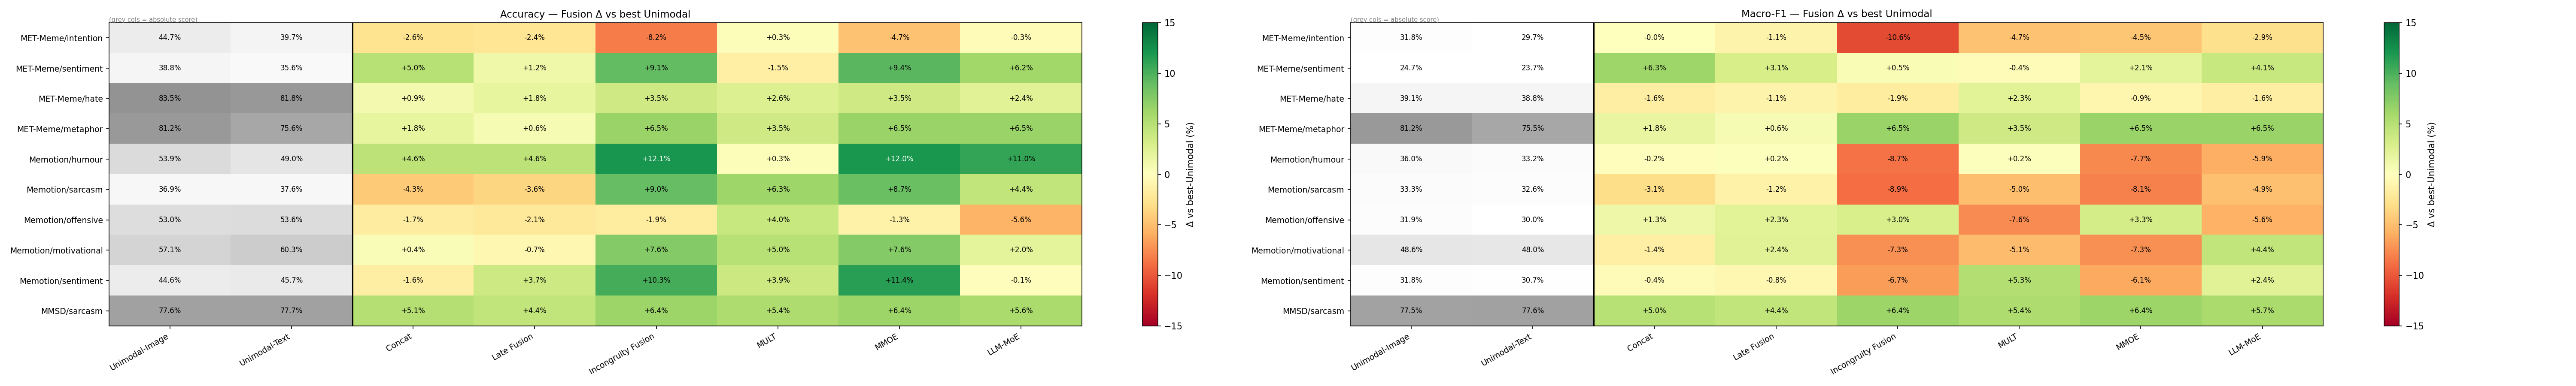
\includegraphics[width=\linewidth]{figures/moe_full_heatmap.png}
  \caption{Accuracy delta of each fusion method relative to the best unimodal baseline
  (green = improvement, red = regression). Incongruity Fusion and FusionMoE show consistent
  gains on non-literal tasks (metaphor, sarcasm, offensive).}
  \label{fig:heatmap}
\end{figure}

\textbf{Key findings.}

\textbf{Incongruity Fusion excels on conflict-heavy tasks.}
On MET-Meme/metaphor, Incongruity Fusion achieves 87.6\% Macro-F1—a +5.8\% accuracy gain over
the best standard fusion (Concat) and +12.0\% over Unimodal-Text. This is the most semantically
incongruent task in our benchmark, validating the core hypothesis that explicit conflict modeling
is necessary for non-literal affect. On MMSD/sarcasm, Incongruity Fusion achieves 84.0\% F1,
matching FusionMoE and outperforming Concat by +1.4\%.

\textbf{FusionMoE achieves the best balance across diverse tasks.}
FusionMoE achieves the best or tied-best trained model on 5/10 tasks (MET/hate, MET/metaphor,
Memotion/offensive, Memotion/sentiment, MMSD/sarcasm). Its advantage is most pronounced on tasks
with mixed interaction types, where routing adaptively selects between redundancy, uniqueness, and
synergy experts per sample.

\textbf{Standard fusion can regress on literal tasks.}
On Memotion/humour, Late Fusion outperforms Incongruity Fusion by +8.9\% F1. This is consistent
with our theory: when humor is coded at a coarse level, the classifier benefits more from pooling
shared semantic content than from explicitly modeling the conflict vector. The incongruity signal
introduces noise when the task does not require conflict exploitation.

\textbf{LLMs excel at open-ended tasks but fail on structured affect.}
LLMs achieve the best overall accuracy on MET/intention (o4-mini: 56\%) and Memotion/sarcasm
(Qwen3: 49\% F1), tasks that benefit from commonsense reasoning. However, trained models
outperform all LLMs on MET/metaphor (+14.5\% F1), Memotion/motivational (+14.2\% acc), and
Memotion/sentiment (+27.1\% acc), where nuanced distribution modeling matters more than reasoning.

% ─────────────────────────────────────────────────────────────────────────────
\subsection{Phase 3: Tri-Modal Alignment Study}

Table~\ref{tab:rq2} shows the impact of adding audio as a third modality.

\begin{table}[h]
\centering
\caption{Sentiment and intention accuracy under different fusion configurations. Naive tri-modal
fusion yields zero improvement; the linear projector unlocks audio's contribution.}
\label{tab:rq2}
\begin{tabular}{lcc}
\toprule
\textbf{Configuration} & \textbf{Sentiment Acc} & \textbf{Intention Acc} \\
\midrule
V only                                     & 0.15 & 0.38 \\
V + T (baseline)                           & 0.27 & 0.45 \\
V + T + A (naive, all 9 settings)          & 0.27 & 0.45 \\
\midrule
V + T + A\textsubscript{proj} (projected)  & \textbf{0.82} & \textbf{0.49} \\
\bottomrule
\end{tabular}
\end{table}

\textbf{Key findings.}
Naive V+T+A fusion yields zero improvement over V+T across all 9 prosody variants, due to
modality-space incompatibility between Emotion2Vec and ImageBind.
A learned linear projector bridges this gap, lifting sentiment accuracy from 0.27 to 0.82 (+0.55).
The gain reflects alignment rather than generalization, but the finding is diagnostic:
\emph{audio carries affective signal; the modality gap, not a lack of signal, is the barrier to fusion}.

% ─────────────────────────────────────────────────────────────────────────────
\subsection{Discussion and Error Analysis}

A detailed error analysis—including failure cases for Incongruity Fusion, LLM vs.\ trained model
trade-offs, and limitations of current audio embedding models—is provided in
Appendix~\ref{sec:error_analysis}.

\section{Conclusion and Future Directions}

We presented \textbf{MemeSonic}, a unified system for affective meme understanding and expressive
audio generation. Our central contribution is the operationalization of \emph{cross-modal
incongruity}—the intentional semantic conflict between meme image and text—as a continuous,
differentiable signal that drives both fusion routing and TTS prosody conditioning.

\textbf{Main findings.}
(1) Explicit incongruity modeling improves classification on non-literal affect tasks by up to
+12.1\% accuracy and +14.5\% Macro-F1 over standard fusion, with the largest gains on
metaphor and sarcasm—exactly the tasks where cross-modal conflict is semantically load-bearing.
(2) Incongruity-conditioned audio generation raises pragmatic appropriateness from AMOS 1.68
(Vanilla TTS) to 3.95, with 84.5\% human preference, demonstrating that the pragmatic signal
latent in image-text incongruity can be successfully translated into expressive prosody.
(3) Audio modality carries non-redundant affective information (KL $V\leftrightarrow A = 1.14$
vs.\ KL $V\leftrightarrow T = 0.69$), but naive fusion fails entirely due to modality-space
incompatibility rather than absence of signal—a distinction with practical implications for the
design of tri-modal systems.

\textbf{Limitations.}

\emph{Scale.}
Our models rely on frozen CLIP ViT-B/32 embeddings and may underperform on tasks requiring
fine-grained cultural knowledge. The tri-modal alignment study covers only 100 memes, so the
+0.55 accuracy gain from the linear projector should be read as a diagnostic rather than a
deployable result. Human audio evaluation is likewise small (12 raters, 84 ratings).

\emph{Data quality and annotation subjectivity.}
Sarcasm and humor benchmarks (e.g., Memotion, MMSD) are not meme-domain specific and reflect
social-media text annotation conventions. Within meme datasets, most prior work targets hate
speech—a comparatively low-subjectivity task—while humor intensity and sarcasm type exhibit
substantial inter-annotator disagreement, consistent with our low F1 on humour (36.2\%) and
sarcasm (33.3\%). No existing benchmark jointly annotates sentiment, humor, sarcasm, and audio
for the same memes, precluding end-to-end tri-modal evaluation.

\textbf{Future directions.}
\emph{(1) Meme-specific dataset construction.}
The most impactful near-term contribution would be a large-scale, meme-native dataset with
multi-dimensional affective annotations—sentiment, humor type, sarcasm mechanism, incongruity
score, and paired voiced audio—collected with rigorous inter-annotator agreement protocols.
Such a resource would enable both training and evaluation of the full MemeSonic pipeline without
relying on heterogeneous benchmarks.

\emph{(2) Generalization to broader incongruity domains.}
The incongruity-aware framework developed here is not inherently meme-specific. Sarcasm and humor
in news captions, social media posts, political cartoons, and video shorts share the same
image-text conflict structure. Extending MemeSonic to these domains—particularly short-form video
where temporal incongruity (e.g., a cheerful musical score against distressing imagery) is
prevalent—would demonstrate the generality of the incongruity signal as an architectural primitive.

\emph{(3) Interactive user studies with human-in-the-loop audio creation.}
Rather than passive preference ratings, future work should engage users as active participants in
meme audio creation. A demo-based study could present the meme alongside a palette of prosodically
distinct audio options—spanning emotional tones, speech rates, and incongruity levels—and ask users
to select, remix, or record their preferred voicing. Aggregating these choices would yield
naturalistic, intent-labeled prosody data far richer than post-hoc MOS ratings. Such a study could
also surface cultural and individual variation in how incongruity is perceived and performed,
motivating personalized prosody adaptation grounded in demonstrated user preference rather than
inferred affective labels.

\emph{(4) Joint tri-modal pre-training.}
Our tri-modal alignment study reveals a fundamental obstacle: ImageBind, despite being trained to
bind image, text, and audio in a shared space, produces near-zero cosine similarity between its
audio embeddings and TTS-synthesized speech (Top-1 accuracy $\approx 0\%$), because its audio
encoder was trained on natural soundscapes rather than expressive speech. Bridging this gap with a
post-hoc linear projector yields only a modest +0.55 accuracy improvement, suggesting that
surface-level alignment is insufficient. A more principled fix is to train a shared encoder on
meme image, text, and voiceover audio simultaneously—using incongruity-weighted contrastive
learning as a pre-training objective—so that the resulting embeddings natively support tri-modal
fusion without relying on incompatible pretrained representations.

\emph{(5) LLM + incongruity as structured input.}
Providing the incongruity score $\delta$ and per-modality emotion distributions as structured
features to an LLM (via function calling or tool use) could combine the commonsense reasoning
advantage of large models with the explicit conflict signal of our architecture, potentially
closing the remaining gap on tasks like intention and sarcasm where LLMs currently outperform
trained models.

MemeSonic demonstrates that meme understanding requires moving beyond the assumption of cross-modal
agreement, and that the \emph{conflict itself} is the signal. We hope this work encourages the
community to treat incongruity not as noise to be averaged away, but as a first-class feature to
be modeled, routed on, and generated from.

\appendix

\section{Demo and Resources}
\label{sec:demo}

A live demo of the MemeSonic pipeline—including meme input, incongruity score visualization,
and synthesized audio playback—is available at:

\begin{center}
  \url{https://tinyurl.com/4schzjb5}
\end{center}

The demo allows users to upload a meme image with caption, inspect the per-modality emotion
distributions and computed incongruity score $\delta$, and listen to the three audio variants
(Vanilla TTS, Label-Guided, and MemeSonic).

Generated audio samples from our 100-meme evaluation set are available on Google Drive,
organized by sentiment class and voice setting:

\begin{center}
  \url{https://drive.google.com/drive/folders/1fuWLJP8FWZz0klj3jQmOCMFVCminqf46?usp=sharing}
\end{center}

% ─────────────────────────────────────────────────────────────────────────────
\section{Full Classification Results}
\label{sec:full_results}

Table~\ref{tab:full_acc} reports Accuracy (complementing the Macro-F1 in Table~\ref{tab:main_results})
across all methods and tasks. Table~\ref{tab:llm_vs_trained} and Figure~\ref{fig:llm_heatmap}
provide a direct Macro-F1 comparison between LLM zero-shot baselines and our best trained model
per task, isolating where each paradigm has an advantage.

\begin{table}[h]
\centering
\caption{Accuracy across all methods and tasks. Format mirrors Table~\ref{tab:main_results}.
\best{Bold green} = best trained model; LLM baselines shown for reference.}
\label{tab:full_acc}
\resizebox{\textwidth}{!}{%
\begin{tabular}{llccccccc|ccccc}
\toprule
 & & \multicolumn{7}{c|}{\textbf{Trained Models}} & \multicolumn{5}{c}{\textbf{LLM Zero-Shot}} \\
\cmidrule(lr){3-9}\cmidrule(lr){10-14}
Dataset & Task & Uni-I & Uni-T & Concat & Late & Incong & MULT & MMOE
        & GPT-4o & Gemini & o4-mini & Gemini-CoT & Qwen3 \\
\midrule
MET-Meme & intention  & 40.3 & 38.5 & 40.1 & 39.8 & 28.1 & 36.2 & 34.7
                      & 44.6 & 42.9 & \textbf{56.0} & 37.1 & 52.0 \\
MET-Meme & sentiment  & 29.4 & 28.2 & 36.8 & 33.1 & 30.5 & 29.0 & 31.9
                      & 33.6 & 38.8 & 39.6 & 45.9 & 35.9 \\
MET-Meme & hate       & \best{87.1} & 85.4 & 83.7 & 84.9 & 83.2 & 85.6 & 85.6
                      & 72.7 & 79.4 & 81.7 & 72.1 & 74.6 \\
MET-Meme & metaphor   & 81.2 & 75.5 & 82.9 & 81.8 & \best{87.6} & 84.7 & \best{87.6}
                      & 36.7 & 71.3 & 73.1 & 63.5 & 57.1 \\
\midrule
Memotion & humour     & 53.9 & 51.4 & 53.4 & \best{54.3} & 45.8 & 52.0 & 46.9
                      & 43.1 & 49.3 & 48.0 & 38.3 & 50.9 \\
Memotion & sarcasm    & \best{55.7} & 55.2 & 52.4 & 54.9 & 46.1 & 49.8 & 47.3
                      & 46.6 & 58.6 & 63.1 & 58.3 & 67.0 \\
Memotion & offensive  & 50.6 & 48.7 & 53.1 & 54.8 & 55.3 & 42.1 & \best{56.0}
                      & 42.1 & 50.2 & 76.4 & 49.3 & 46.3 \\
Memotion & motivational & 67.1 & 66.3 & 65.9 & \best{69.3} & 60.8 & 62.9 & 61.7
                        & 54.9 & 55.0 & 55.1 & 54.7 & 55.0 \\
Memotion & sentiment  & 57.3 & 55.9 & 56.8 & 56.5 & 49.4 & \best{62.7} & 50.3
                      & 50.1 & 45.7 & 50.8 & 43.9 & 40.0 \\
\midrule
MMSD 2.0 & sarcasm    & 77.5 & 77.6 & 82.6 & 82.0 & \best{84.0} & 83.0 & \best{84.0}
                      & 80.0 & 85.9 & 84.0 & 74.0 & 57.2 \\
\bottomrule
\end{tabular}}
\end{table}

\begin{figure}[h]
  \centering
  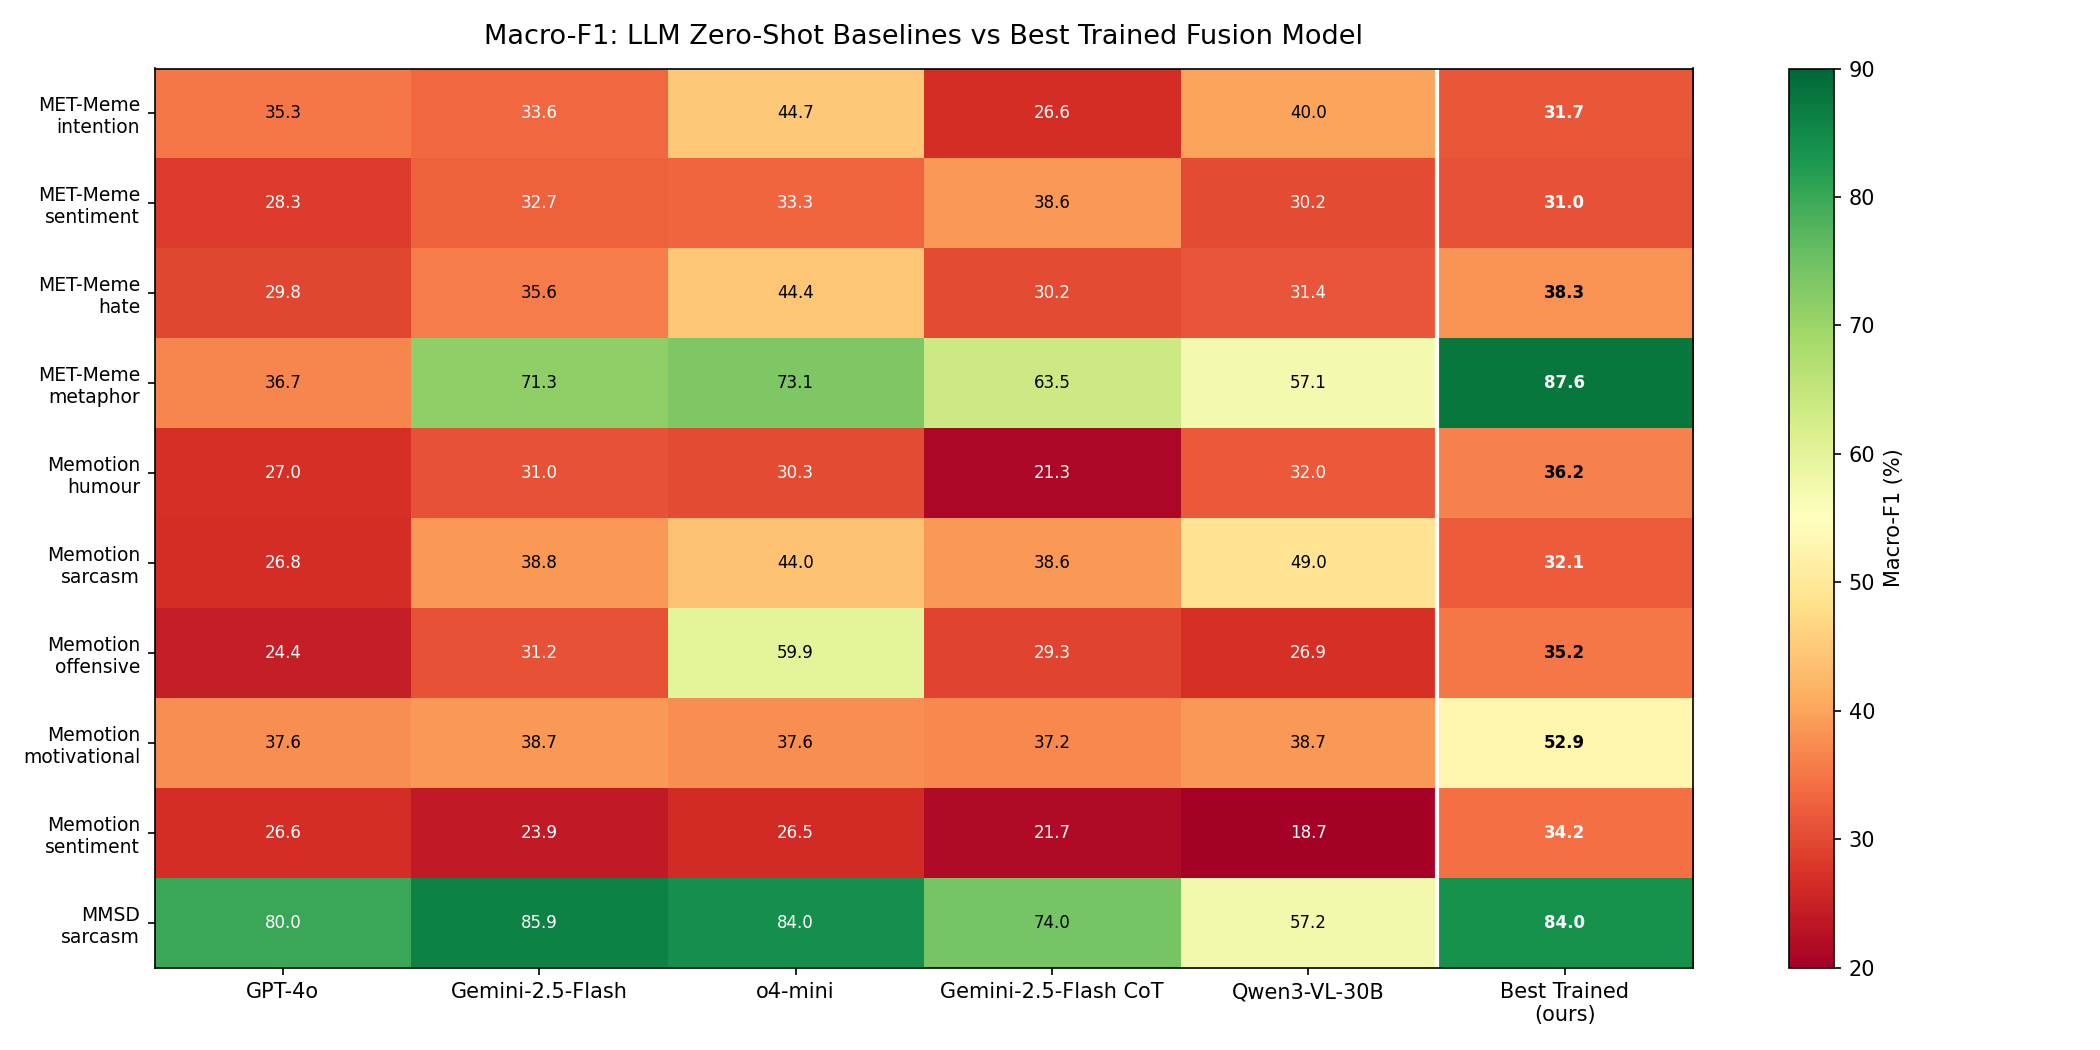
\includegraphics[width=\linewidth]{figures/llm_vs_trained_f1_heatmap.png}
  \caption{Macro-F1 gap between the best LLM zero-shot baseline and the best trained model per task.
  Green = trained model wins; red = LLM wins. Trained models dominate on structured non-literal tasks
  (metaphor, motivational, sentiment); LLMs dominate on open-ended reasoning tasks (intention, sarcasm).}
  \label{fig:llm_heatmap}
\end{figure}

% ─────────────────────────────────────────────────────────────────────────────
\section{t-SNE Visualization of Audio Embeddings}
\label{sec:tsne}

Figure~\ref{fig:tsne} shows a t-SNE projection of Emotion2Vec embeddings for all 900 audio
samples (100 memes $\times$ 9 voice settings), colored by ground-truth sentiment class.
Points cluster by sentiment rather than by voice setting, confirming that Emotion2Vec captures
semantic emotion content and is largely insensitive to surface prosodic variation (pitch, rate,
stability) introduced by different ElevenLabs voice settings.

\begin{figure}[h]
  \centering
  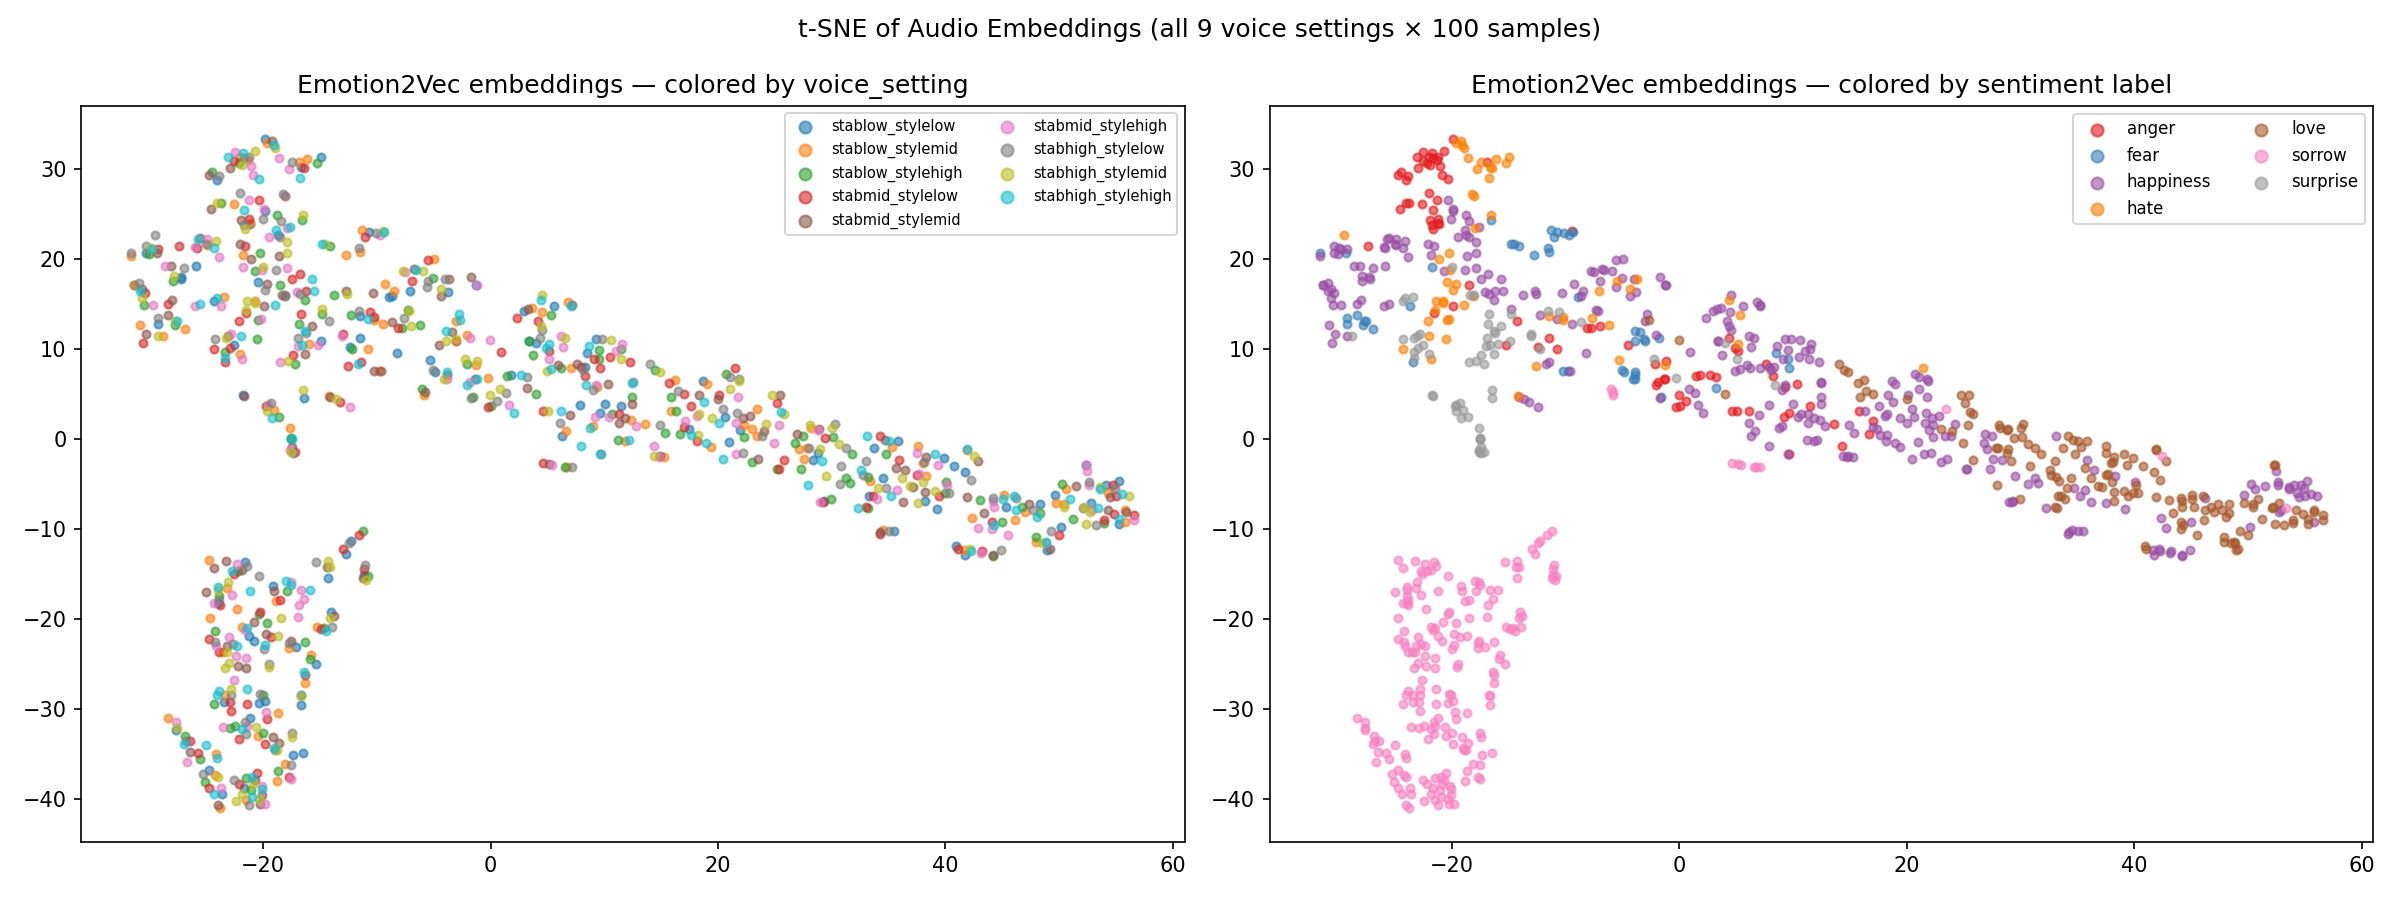
\includegraphics[width=0.85\linewidth]{figures/tsne_audio_embeddings.png}
  \caption{t-SNE of Emotion2Vec embeddings for 900 audio files (100 memes $\times$ 9 prosody settings).
  Colors indicate GT sentiment class. Clustering by sentiment rather than voice setting confirms
  Emotion2Vec's robustness to prosodic surface variation.}
  \label{fig:tsne}
\end{figure}

% ─────────────────────────────────────────────────────────────────────────────
\section{Prosody Grid Details}
\label{sec:prosody_grid}

The 9-point prosody grid used in the tri-modal alignment study spans:
\[
  \text{stability} \in \{0.2,\,0.5,\,0.8\} \;\times\; \text{style} \in \{0.2,\,0.5,\,0.8\}
\]
using ElevenLabs \texttt{voice\_settings}. All other parameters (\texttt{similarity\_boost}=0.75,
\texttt{use\_speaker\_boost}=True) are held constant. Table~\ref{tab:prosody_grid} summarizes
the intended perceptual effect of each setting combination.

\begin{table}[h]
\centering
\caption{Prosody grid: perceptual intent of each (stability, style) combination.}
\label{tab:prosody_grid}
\begin{tabular}{cc p{8cm}}
\toprule
\textbf{Stability} & \textbf{Style} & \textbf{Perceptual character} \\
\midrule
0.2 & 0.2 & Unstable, flat — inconsistent emotion, low expressiveness \\
0.2 & 0.5 & Unstable, moderate — variable rhythm, some emotional coloring \\
0.2 & 0.8 & Unstable, expressive — erratic and emotionally intense \\
0.5 & 0.2 & Neutral, flat — consistent but monotone (close to vanilla TTS) \\
0.5 & 0.5 & Balanced — moderate stability and expressiveness \\
0.5 & 0.8 & Neutral stability, high style — expressive with controlled variation \\
0.8 & 0.2 & Very stable, flat — robotic, minimal affect \\
0.8 & 0.5 & Stable, moderate — clear and measured delivery \\
0.8 & 0.8 & Stable, expressive — polished and emotionally rich \\
\bottomrule
\end{tabular}
\end{table}

% ─────────────────────────────────────────────────────────────────────────────
\section{Dataset Statistics}
\label{sec:dataset_stats}

Table~\ref{tab:dataset_stats} summarizes the dataset splits and class distributions used in
Phase~1 experiments.

\begin{table}[h]
\centering
\caption{Dataset statistics for Phase~1 benchmarks.}
\label{tab:dataset_stats}
\begin{tabular}{llcccl}
\toprule
\textbf{Dataset} & \textbf{Task} & \textbf{Train} & \textbf{Val} & \textbf{Test} & \textbf{Classes} \\
\midrule
MET-Meme  & intention    & 1{,}400 & 300 & 340 & 5 (interactive, expressive, entertaining, offensive, other) \\
MET-Meme  & sentiment    & 1{,}400 & 300 & 340 & 7 (happiness, love, anger, sorrow, fear, hate, surprise) \\
MET-Meme  & hate         & 1{,}400 & 300 & 340 & 4 (intensity levels) \\
MET-Meme  & metaphor     & 1{,}400 & 300 & 340 & 2 (binary) \\
\midrule
Memotion  & humour       & 5{,}593 & 699 & 700 & 3 \\
Memotion  & sarcasm      & 5{,}593 & 699 & 700 & 3 \\
Memotion  & offensive    & 5{,}593 & 699 & 700 & 4 \\
Memotion  & motivational & 5{,}593 & 699 & 700 & 2 \\
Memotion  & sentiment    & 5{,}593 & 699 & 700 & 3 (pos/neu/neg) \\
\midrule
MMSD 2.0  & sarcasm      & 16{,}000 & 3{,}000 & 3{,}482 & 2 (binary) \\
\bottomrule
\end{tabular}
\end{table}


% ── References ─────────────────────────────────────────────────────────────────
\bibliographystyle{abbrvnat}
\bibliography{references}

\end{document}
